% $Id: whatis.tex,v 1.2 2003/02/17 00:25:21 jasta Exp $
% Copyright (c) 2002, The giFT Project
% written by Eelco Lempsink (eelco@wideview.33lc0.net)

\documentclass[10pt]{article}

\usepackage{url}
\usepackage{hyperref}
\usepackage[dvips]{graphicx}

\setlength{\parindent}{0pt}

\begin{document}

\begin{center}
\textsf{\textbf{\Huge{giFT}\\ \huge{What is the giFT project?}\\
\normalsize{Last update: \today}}}
\end{center}

\tableofcontents

\setlength{\parskip}{1.4ex}

\section{About this document}
Many people are puzzled about the structure of the giFT project. Questions
such as "What is giFT?" and "What is OpenFT?" are not easily answered. This
document will try to make everything clear. For generic questions, or questions
more vaguely related to the giFT project, you should read the
\href{http://gift.sourceforge.net/docs.php?document=faq.html}{FAQ} instead.

\section{What is giFT?}
giFT is like a 'bridge'. It's a daemon (a program that runs in the background
without active Input/Output) that can handle multiple file sharing protocols.
The protocols will be dynamically loaded as a sort of 'plugin'.  That's one
side of the bridge.

\begin{figure}[bh]
  \begin{center}
    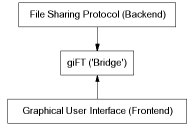
\includegraphics[scale=0.5]{bridge}
  \end{center}
  \caption{giFT works like a 'bridge'}
\end{figure}

The other side of the bridge is a simple interface protocol, which provides the
frontend (also called 'GUI' or 'interface') a unified method to work with all
file sharing protocols.  In the near future we will also provide a clean C API
for communicating with the giFT daemon via libgift so that knowledge of the
specific protocol or even network programming in general will not be required.

\section{What is OpenFT?}
OpenFT is a file sharing protocol developed by the giFT project. It is loosely
based on the idea of FastTrack, working in a different way to well-known file
sharing programs like Napster and Gnutella.

Napster (and OpenNap) work with one server providing users a way to share files
and search for files from other users, in a big list. This requires constantly
running servers, and bringing the network down is as easy as shutting those
(few) servers down. Also, those servers must be able to handle thousands
of connections, and must have lots of memory and disk space to maintain and
search the filelists.

Gnutella creates a structure of 'nodes' (computers connected to the network),
with every node connecting to a few others. Search requests must be forwarded
through the whole network (or at least a large part of it). Because of this,
Gnutella uses a lot of bandwidth, and it can take a long time to recieve search
requests.

\begin{figure}[bh]
  \begin{center}
    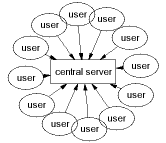
\includegraphics[scale=0.5]{napster}
    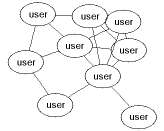
\includegraphics[scale=0.5]{gnutella}
  \end{center}
  \caption{Napster and Gnutella}
\end{figure}

OpenFT combines the idea of Napster and Gnutella, making a network of nodes
connected to each other, but with certain nodes having specific tasks. There are
3 different kind of nodes.
\begin{itemize}
\item{USER}\\
The 'normal' nodes are USER nodes, they don't have any special function.
%, but they'll exchange nodes lists when connection to other nodes. (???)
\item{SEARCH}\\
These nodes handle search requests. They search the filelists their CHILD
nodes (explained below) submitted to them. These nodes must have a capable
Internet connection and at least 128M RAM.  A modern processor is highly
recommended as well.
\item{INDEX}\\
Nodes with a fast connection and lots of memory should be INDEX nodes. INDEX
nodes keep lists of available search nodes, collect statistics, and try to
maintain the structure of the network.
\end{itemize}

A node can be both a SEARCH and a INDEX node.

USER nodes will pick three SEARCH nodes to be their PARENT nodes. They'll
submit their shares list to them if the PARENT accepts the USER as its CHILD.
By default, SEARCH nodes will be PARENTS for a maximum of 500 CHILD nodes.

\begin{figure}[ht]
  \begin{center}
    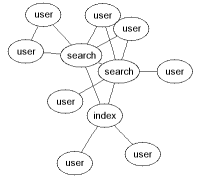
\includegraphics[scale=0.5]{openft}
  \end{center}
  \caption{OpenFT}
\end{figure}

For more technical information about OpenFT, you must read the source code,
because there's no document covering that at the moment. Also, you can use
\href{http://doxygen.org}{Doxygen} to generate documentation from comments in
the source files, using doxygen/doxygen.conf in the CVS repository.

When we (members of the giFT project) say 'OpenFT', we can mean two different
things. First, there is the OpenFT \textbf{protocol}, but there's also OpenFT
as an \textbf{implementation} in the form of a plugin for giFT. Keep that in
mind.

\section{What is the relation between giFT and OpenFT?}
This is a frequently misunderstood issue. As you know, if you've read the
document this far, giFT and OpenFT are two different projects started by the
giFT project. That's about the only thing they have in common.

giFT is a program that works like a 'bridge'.\\
OpenFT is a network protocol \textbf{and} a plugin for giFT, implementing the
OpenFT protocol.

Because both giFT and OpenFT were developed by the giFT project, and the
programs are distributed together, we often call it "giFT/OpenFT". If giFT gets
a OpenNap plugin, giFT together with that plugin (probably) will be called
giFT/OpenNap.

If you referrer to giFT/OpenFT just as "OpenFT" you're incorrect. For instance,
we had people coming to us, claiming they wanted to implement OpenFT, when they
actually meant they wanted to write a frontend for giFT, to use OpenFT.

When you want to share files on OpenFT, you'll have to do that \textbf{through}
giFT. That means you tell giFT what files you want to share, and giFT will pass
that info to the different plugins. Similary for searching, downloading, etc.

\section{What is the relation of a frontend to giFT?}
giFT offers the frontend a unified way to communicate with OpenFT and other
file sharing protocols. This way you can make a frontend and only have to teach
it one 'trick', namely using and understanding the giFT interface protocol.

For more information about this protocol, read the
\href{http://gift.sourceforge.net/docs.php?document=interface.html}{Interface
Protocol Documentation}.

giFT relies on third party frontends. Luckily, quite a few already exist. A
\href{http://gift.sourceforge.net/dev/clients.php}{list of clients} is
available on our website.

\section{What is the relation of a frontend to OpenFT?}
Hah! There is none! A frontend doesn't have to know anything about OpenFT, and
it must use giFT for communicating with it. There is no way for a frontend to
communicate directly with OpenFT, because you'll have to implement everything
that giFT does into it, to achieve that. And that would be rather silly,
wouldn't it?

\end{document}
